\documentclass{article}

\usepackage{amsmath}
\usepackage{relsize}
\usepackage{tikz}
\usepackage{setspace}
\usepackage{float}
\usepackage[a4paper, margin = 3cm]{geometry}



\begin{document}
\fontsize{14pt}{0}
\onehalfspacing

\begin{titlepage}
    \begin{center}
        \vspace*{1cm}

        \textbf{RESUME MATA KULIAH VARIABEL KOMPLEKS}

        \vspace{0.5cm}
        \textit{Resume ini diajukan untuk mememenuhi salah satu Tugas Akhir Mata Kuliah Variabel Kompleks}

        \vspace{1.5cm}
        
\includegraphics[width=0.5\textwidth]{Telkom University Logo.png}

        \vspace{1.5cm}
        \textbf{Kelompok 1 TT4502:}\\
        \begin{table}[H]
            \begin{center}
                \begin{tabular}{ll}
                    Erni Dianti            & (1101213192) \\
                    Rangga Aditia Permana  & (1101210019)\\
                    Reynaldhi Tryana Graha & (1101213117) \\
                    Shasyabilla Ardita H   & (1101210455)
                    \end{tabular}
                \end{center}
            \end{table}
        \vfill
        \textbf{
            FAKULTAS TEKNIK ELEKRO\\
            TELKOM UNIVERSITY\\
            BANDUNG\\
            2023
        }
        \vspace*{1cm}
    \end{center}
\end{titlepage}

\begin{center}
    \textbf{BILANGAN KOMPLEKS}
\end{center}
\leavevmode\\

Bilangan Kompleks adalah bilangan yang dapat direpresentasikan sebagai \( x + iy \), dimana $x$ dan $y$ adalah bilangan real ($R$) dan $i$ adalah suatu bilangan imaginer dimana \( i = \sqrt{-1} \) dan \( i^2 = -1 \).\\

Bilangan Kompleks biasanya ditulis dalam bentuk:
\begin{align}
    \boxed{z = x + iy}\nonumber
\end{align}

\>dimana,
\begin{itemize}
    \item $x$ adalah bagian $Re(z)$, dan
    \item $y$ adalah bagian $Im(z)$. \\
\end{itemize}

Contoh:
\begin{align}
    z & = 6 + \sqrt{-16}
    \nonumber                            \\
      & = 6 + \sqrt{-1} \times \sqrt{16}
    \nonumber                            \\
      & = 6 + i \times 4
    \nonumber                            \\
      & = 6 + 4i
    \nonumber
\end{align}

maka:
\begin{itemize}
    \item $Re(z) = 6$, dan
    \item $Im(z) = 4$. \\ \\ \\ \\
\end{itemize}



\newpage
\begin{center}
    \textbf{Notasi Bilangan Kompleks}
\end{center}
\leavevmode\\

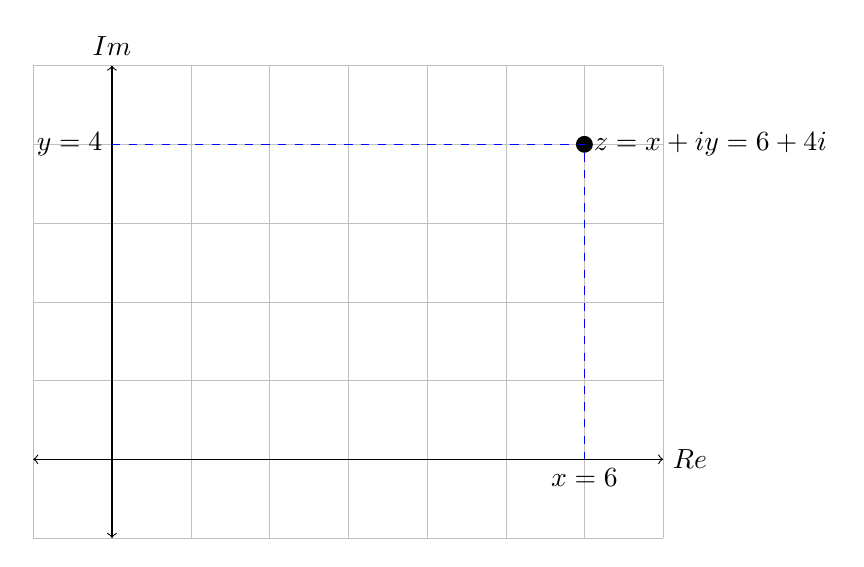
\begin{tikzpicture}
    \draw [ultra thin, lightgray] (-1,-1) grid (7,5);
    \draw [<->] (-1, 0) -- (7, 0) node[right] {$Re$};
    \draw [<->] (0, -1) -- (0, 5) node[above] {$Im$};
    \draw [black, fill = black] (6,4) circle [radius = 1 mm]
    node[black, right] {$ z = x + iy = 6 + 4i $};
    \draw [blue, dashed] (0,4) node[black, left] {$ y = 4 $}
    -| (6,0) node[black, below] {$ x = 6 $};
\end{tikzpicture}
\\ \\

Misal $ z_1 = ( x_1 , y_1 )  $ dan $ z_2 = ( x_2 , y_2 ) $, maka berlaku:

\begin{align}
    z_1 + z_2     & = ( x_1 \;,\; y_1 ) + ( x_2 \;,\; y_2 )
    \nonumber                                                       \\
                  & = ( x_1 + x_2 \;,\; y_1 + y_2 )
    \nonumber                                                       \\
    \nonumber                                                       \\
    z_1 \cdot z_2 & = ( x_1 \;,\; y_1 ) \cdot ( x_2 \;,\; y_2 )
    \nonumber                                                       \\
                  & = ( x_1 x_2 - y_1 y_2 \;,\; x_1 y_2 + x_2 y_1 )
    \nonumber                                                       \\
    \nonumber                                                       \\
    a \cdot z_1   & = a \cdot ( x_1 \;,\; y_1 )
    \nonumber                                                       \\
                  & = ( ax_1 \;,\; ay_1 )
    \nonumber
\end{align}



\newpage
\begin{center}
    \textbf{Operasi Aritmatika Pada Bilangan Kompleks}
\end{center}
\leavevmode\\

\begin{enumerate}
    \item   \textbf{Penjumlahan Bilangan Kompleks}\\

          Misalkan dua bilangan kompleks:
          \begin{align}
              z_1 & = a + bi
              \nonumber      \\
              z_2 & = c + di
              \nonumber
          \end{align}

          \begin{itemize}
              \item $z_1 = 0$ jika dan hanya jika $a = 0$ dan $b = 0$
              \item $z_1 = z_2$ jika dan hanya jika $a = b$ dan $b = d$
          \end{itemize}

          \textbf{Contoh:}
          \begin{align}
              2 + 5i = \dfrac{4}{2} + \dfrac{10}{2}i \nonumber
          \end{align}
          \begin{itemize}
              \item Jika $z_1 \neq z_2$ maka $z_1$ tidak dapat dibandingkan lebih besar atau lebih kecil dari $z_2$
          \end{itemize}
          \leavevmode
          \\\\

    \item   \textbf{Perkalian bilangan kompleks dengan skalar}\\

          Jika:
          \begin{align}
              z_1 = (a + bi) \nonumber
          \end{align}

          Maka:
          \begin{align}
              k \cdot z_1 & = k \cdot (a + bi)
              \nonumber                          \\
                          & = ka + kbi \nonumber
          \end{align}

          Contoh:
          \begin{align}
              z_1 & = 2 + 5i
              \nonumber      \\
              k   & = 2
              \nonumber
          \end{align}

          Jawab:
          \begin{align}
              k \cdot z_1 & = 2 \cdot (2 + 5i)
              \nonumber                        \\
                          & = 4 + 10i
              \nonumber
          \end{align}
          \leavevmode
          \newpage
    \item   \textbf{Perkalian dua bilangan kompleks}\\

          Jika:
          \begin{align}
              z_1 & = a + bi
              \nonumber      \\
              z_2 & = c + di
              \nonumber
          \end{align}

          Maka:
          \begin{align}
              z_1 \cdot z_2 & = (a + bi)\cdot(c + di)
              \nonumber                                \\
                            & = (ac - bd) + (ad + bc)i
              \nonumber
          \end{align}

          Contoh:
          \begin{align}
              z_1 & = 1 + 2i
              \nonumber      \\
              z_2 & = 3 + 5i
              \nonumber
          \end{align}

          Jawab:
          \begin{align}
              z_1 \cdot z_2 & = (1 + 2i) \cdot (3 + 5i)
              \nonumber                                 \\
                            & = (3 - 10) + (5 + 6)i
              \nonumber                                 \\
                            & = -7 + 11i
              \nonumber
          \end{align}
          \leavevmode
          \\\\

    \item   \textbf{Pembagian dua bilangan kompleks}\\

          Jika
          \begin{align}
              z_1 & = a + bi
              \nonumber      \\
              z_2 & = c + di
              \nonumber
          \end{align}

          Maka $\dfrac{z_1}{z_2}$ menyatakan pembagian bilangan kompleks dengan pembilang $z_1$ dan penyebut $z_2$. Penyebut dikalikan sekawannya $\dfrac{z_1}{z_2} \cdot \dfrac{?}{z_2}$. Agar nilai semula tidak berubah, maka pembilang juga harus dikalikan dengan bilangan yang sama: $\dfrac{z_1}{z_2} \cdot \dfrac{\overline{z_2}}{z_2}$. Sekarang pembilang bernilai riil dan pembagian dapat dilakukan.

          \newpage
          Contoh:
          \begin{align}
              z_1 & = 1 + 2i
              \nonumber      \\
              z_2 & = 2 + 3i
              \nonumber
          \end{align}

          Maka:
          \begin{align}
              \dfrac{z_1}{z_2} & = \dfrac{1+2i}{2+3i}
              \nonumber                                                        \\
                               & = \dfrac{1+2i}{2+3i} \cdot \dfrac{2-3i}{2-3i}
              \nonumber                                                        \\
                               & = \dfrac{(2+6)+(-3+4)i}{2^2+3^2}
              \nonumber                                                        \\
                               & = \dfrac{8}{13} + \dfrac{1}{13}i
              \nonumber
          \end{align}
\end{enumerate}



\newpage
\begin{center}
    \textbf{Modulus Bilangan Kompleks}
\end{center}
\leavevmode\\

Modulus atau nilai absolut bilangan kompleks $ z = x + iy $, didefinisikan sebagai bilangan real tidak negatif yang merupakan panjang vektor posisi dari $z$ (jarak antara $z$ dengan pusat sumbu).
\\ \\

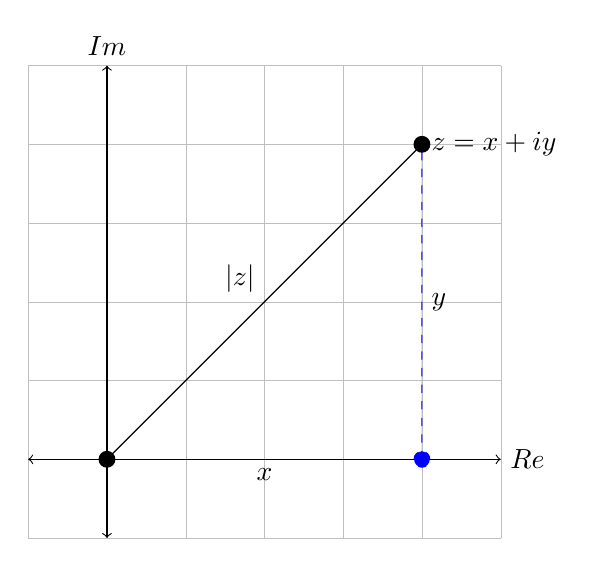
\begin{tikzpicture}
    \draw [ultra thin, lightgray] (-1,-1) grid (5,5);
    \draw [<->] (-1, 0) -- (5, 0) node[right] {$Re$};
    \draw [<->] (0, -1) -- (0, 5) node[above] {$Im$};
    \draw [black, fill = black] (4,4) circle [radius = 1 mm]
    node[black, right] {$ z = x + iy $};
    \draw [black, fill = black] (0,0) circle [radius = 1 mm] -- (4,4);
    \draw [dashed, blue, fill = blue] (4,0) circle [radius = 1 mm] -- (4,4);
    \draw (2,2) node[above, anchor=south east, black] {$|z|$};
    \draw (4,2) node[right, black] {$y$};
    \draw (2,0) node[below, black] {$x$};
\end{tikzpicture}
\\ \\

\begin{align}
    |z|         & = \sqrt{x^2+y^2}
    \nonumber                                        \\
    \nonumber                                        \\
    |z_1 - z_2| & = \sqrt{(x_1-x_2)^2 + (y_1-y_2)^2}
    \nonumber
\end{align}
\\ \\

Sifat Modulus
\begin{align}
    \bigg | \frac{z_1}{z_2} \bigg | & = \frac{|z_1|}{|z_2|}
    \nonumber                                               \\
    \nonumber                                               \\
    |z_1 z_2|                       & = |z_1| \cdot |z_2|
    \nonumber
\end{align}
\\ \\



\newpage
\begin{center}
    \textbf{Sekawan/\textit{Konjugate} Bilangan Kompleks}
\end{center}
\leavevmode\\

Misalkan $ z = x + iy $, sekawan dari $z$ (notasi = $\overline{z}$) adalah pencerminan dari $z$ terhadap sumbu real ($R$).
\\ \\

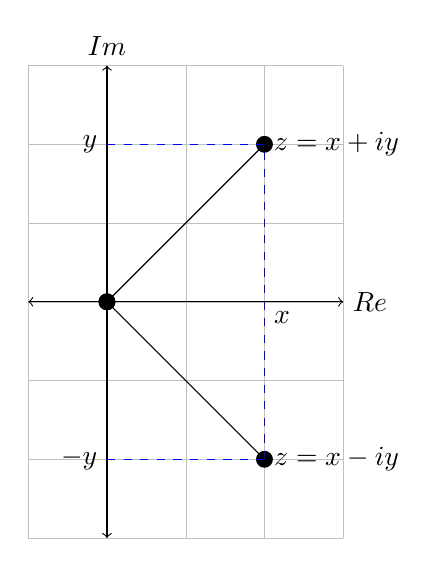
\begin{tikzpicture}
    \draw [ultra thin, lightgray] (-1,-3) grid (3,3);
    \draw [<->] (-1, 0) -- (3, 0) node[right] {$Re$};
    \draw [<->] (0, -3) -- (0, 3) node[above] {$Im$};
    \draw [black, fill = black] (2,2) circle [radius = 1 mm]
    node[black, right] {$ z = x + iy $};
    \draw [black, fill = black] (2,-2) circle [radius = 1 mm]
    node[black, right] {$ z = x - iy $};
    \draw [black, fill = black] (0,0) circle [radius = 1 mm] -- (2,2);
    \draw [black, fill = black] (0,0) circle [radius = 1 mm] -- (2,-2);
    \draw [dashed, blue] (2,-2) -- (2,2);
    \draw [dashed, blue] (0,2) node[left, black] {$y$} -- (2,2);
    \draw [dashed, blue] (0,-2) node[left, black] {$-y$} -- (2,-2);
    \draw (2,0) node[below right, black] {$x$};
\end{tikzpicture}
\\ \\ \\ \\

Sifat Sekawan/\textit{Konjugate}:
\begin{itemize}
    \item $\overline{z_1 + z_2} = \overline{z_1} + \overline{z_2}$
    \item $\overline{z_1 z_2} = \overline{z_1} \cdot \overline{z_2}$
    \item $|z| = \overline{z}$
    \item $\overline{zz} = |z|^2$
    \item $Re(z) = \dfrac{z+z}{2}$\\ \\
          $Im(z) = \dfrac{z-z}{2i}$
\end{itemize}



\newpage
\begin{center}
    \textbf{Representasi Polar}
\end{center}
\leavevmode\\

Misalkan $r$ dan adalah koordinat polar dari titik $(x, y)$ bilangan kompleks bukan nol $z = x + iy$. Karena $x = r cos \theta $ dan $y = r sin \theta$, maka bilangan Kompleks $z$ dapat
ditulis dalam bentuk polar:

\begin{align}
    z & = r(cos \theta + i sin \theta)
    \nonumber                          \\
    \nonumber                          \\
    z & = r \angle \theta
    \nonumber
\end{align}

dengan,
\begin{itemize}
    \item r adalah modulus dari $z$:\\
          $ r = |z| = \sqrt{x^2+y^2} $
    \item $\theta$ adalah argumen dari $z$:\\
          $ \theta = tan^{-1} \bigg(\dfrac{y}{x}\bigg) $
\end{itemize}
\leavevmode\\

Contoh:
\begin{align}
    z = 3 + 4i \nonumber
\end{align}

Modulus:
\begin{align}
    r & = \sqrt{a^2 + b^2}
    \nonumber              \\
      & = \sqrt{3^2 + 4^2}
    \nonumber              \\
      & = 5
    \nonumber
\end{align}

Argumen:
\begin{align}
    \theta & = tan^{-1} \dfrac{b}{a}
    \nonumber                        \\
           & = tan^{-1} \dfrac{4}{3}
    \nonumber                        \\
           & = 53,1^{\circ}
    \nonumber
\end{align}

\begin{align}
    z & = 3 + 4i
    \nonumber                                      \\
      & = 5(\cos 53,1^{\circ} + \sin 53,1^{\circ})
    \nonumber                                      \\
      & = 5 \angle 53,1^{\circ}
    \nonumber
\end{align}



\newpage
\begin{center}
    \textbf{Representasi Euler}
\end{center}
\leavevmode\\

Notasi matematis formal adalah bentuk Euler:
\begin{align}
    \boxed{z = re^{i\theta}}
    \nonumber
\end{align}

Identitas Euler:
\begin{align}
    \boxed{e^{i\theta} = cos\theta + i sin\theta}
    \nonumber
\end{align}
\leavevmode\\

Contoh:
\begin{align}
    z = 3 + 4i \nonumber
\end{align}

Modulus:
\begin{align}
    r & = \sqrt{a^2 + b^2}
    \nonumber              \\
      & = \sqrt{3^2 + 4^2}
    \nonumber              \\
      & = 5
    \nonumber
\end{align}

Argumen:
\begin{align}
    \theta & = tan^{-1} \dfrac{b}{a}
    \nonumber                        \\
           & = tan^{-1} \dfrac{4}{3}
    \nonumber                        \\
           & = 53,1^{\circ}
    \nonumber
\end{align}

\begin{align}
    z                   & = 3 + 4i
    \nonumber                                                        \\
                        & = 5e^{i 53,1^{\circ}}
    \nonumber                                                        \\
    5e^{i 53,1^{\circ}} & = 5(\cos 53,1^{\circ} + \sin 53,1^{\circ})
    \nonumber
\end{align}



\newpage
\begin{center}
    \textbf{Perkalian dan Pangkat Bentuk Exponen}
\end{center}
\begin{align}
    e^{i\theta_1} e^{i\theta_2} & = (cos\theta_1 + i sin\theta_1)(cos\theta_2 + i sin\theta_2)
    \nonumber                                                                                                                                \\
                                & =(cos\theta_1 cos\theta_2 - sin\theta_1 sin\theta_2) + i(sin\theta_1cos\theta_2 + cos\theta_1 sin\theta_2)
    \nonumber                                                                                                                                \\
                                & = cos(\theta_1 + \theta_2) + i\;sin(cos(\theta_1 + \theta_2))
    \nonumber                                                                                                                                \\
                                & = e^{i(\theta_1 + \theta_2)}
    \nonumber
\end{align}

Maka, jika $z_1 = r_1e^{i\theta_1}$ dan $z_2 = r_2e^{i\theta_2}$, produk $z_1z_2$ memiliki bentuk eksponensial:
\begin{align}
    z_1z_2 & = r_1e^{i\theta_1} r_2e^{i\theta_2}
    \nonumber                                    \\
           & = r_1r_2e^{i\theta_1}e^{i\theta_2}
    \nonumber                                    \\
           & = (r_1r_2)e^{i(\theta_1\theta_2)}
    \nonumber
\end{align}
\begin{align}
    \dfrac{z_1}{z_2} & = \dfrac{r_1e^{i\theta_1}}{r_2e^{i\theta_2}}
    \nonumber                                                                                                                           \\
                     & = \dfrac{r_1}{r_2} \cdot \dfrac{r_1e^{i\theta_1}}{r_2e^{i\theta_2}} \cdot \dfrac{e^{-i\theta_2}}{e^{-i\theta_2}}
    \nonumber                                                                                                                           \\
                     & = \dfrac{r_1}{r_2} \cdot \dfrac{e^{i(\theta_1-\theta_2)}}{e^{i0}}
    \nonumber                                                                                                                           \\
                     & = \dfrac{r_1}{r_2} e^{i(\theta_1-\theta_2)}
    \nonumber
\end{align}
\begin{align}
    z^{-1} & = \dfrac{1}{z}
    \nonumber                                \\
           & = \dfrac{1e^{i0}}{re^{i\theta}}
    \nonumber                                \\
           & = \dfrac{1}{r} e^{i(0-\theta)}
    \nonumber                                \\
           & = \dfrac{1}{r} e^{-i\theta}
    \nonumber
\end{align}
\begin{align}
    z^n & = r^n e^{in\theta}
    \nonumber
\end{align}



\newpage
\begin{center}
    \textbf{Fungsi Kompleks}
\end{center}
\leavevmode\\

Fungsi kompleks $f(z)$ menyatakan pemetaan dari bidang kompleks asal $z$ (domain) ke bidang kompleks hasil $w$ (range) dengan suatu pola yang diatur oleh $f(z)$.
\\

Contoh (titik ke titik):
\begin{align}
    f(z)  & = 2z + 1
    \nonumber                 \\
          & = 2(x+iy) + 1
    \nonumber                 \\
          & = 2x + 2iy + 1
    \nonumber                 \\
          & = (2x + 1) + 2iy
    \nonumber                 \\
    \nonumber                 \\
    Re(z) & = u(x,y) = 2x + 1
    \nonumber                 \\
    Im(z) & = v(x,y) = 2y
    \nonumber
\end{align}

Contoh (lintasan ke lintasan):
\begin{align}
    f(z)  & = \overline{z}
    \nonumber              \\
          & = x - iy
    \nonumber              \\
    \nonumber              \\
    Re(z) & = u(x,y) = x
    \nonumber              \\
    Im(z) & = v(x,y) = -y
    \nonumber
\end{align}

Contoh (daerah ke daerah):
\begin{align}
    f(z)    & = z + 1
    \nonumber         \\
    D : |z| & <1
    \nonumber         \\
    f(z)    & = z + 1
    \nonumber         \\
    w       & = z + 1
    \nonumber         \\
    z       & = w - 1
    \nonumber         \\
    |w-1|   & < 1
    \nonumber         \\
    \nonumber
\end{align}
\\

\begin{center}
    \textbf{Titik Singular}
\end{center}
\leavevmode\\

Titik dimana $f(z)$ gagal dipetakan ke titik lain. Contoh pada fungsi $f(z) = \dfrac{1}{z+1}$ gagal dipetakan pada titik asal $z=1$ karena $\dfrac{0}{0}$ tidak terdefinisi.



\newpage
\begin{center}
    \textbf{Limit Fungsi Kompleks}
\end{center}
\leavevmode\\

Konsep limit pada fungsi kompleks $f(z)$ diperluas dari limit pada fungsi real $f(x)$ sebagai:
Pada fungsi kompleks $f(z)$, $\lim_{z \to z_0} f(z)$ bernilai $L$ atau
\begin{align}
    \boxed{\lim_{z \to z_0} f(z) = L}
    \nonumber
\end{align}
jika terdapat $\epsilon  > 0$ dan $\delta  > 0$ sedemikian sehingga jika ada $\epsilon$ yang memenuhi $|f(z) - L| \leq \epsilon$ , maka terilustrasi:
\begin{itemize}
    \item $|z - z_0| \leq \delta$ adalah disk dengan pusat di $z_0$ dan jari-jari $\delta$
    \item $|f(z) - L| \leq \epsilon$ adalah disk dengan pusat di $L$ dan jari-jari $\epsilon$
\end{itemize}
\leavevmode\\ \\

\begin{center}
    \textbf{Turunan Fungsi Kompleks}
\end{center}
\leavevmode\\

Perhitungan turunan $f(z)$ dapat melihat dari kemungkinan notasi $f(z)$:
\begin{itemize}
    \item $f(z)$ dinyatakan secara eksplisit peubah $z$.
    \item $f(z)$ dinyatakan : $f(z) = U(x,y) + iV(x,y)$
    \item $f(z)$ dinyatakan : $f(z) = U(i,\theta)+ iV(i,\theta)$
\end{itemize}
\leavevmode\\

$f(z)$ dinyatakan $f(z) = U(x,y) + iV(x,y)$ dapat diturunkan di $z_0 = x_0 + iy_0$ bila berlaku \textbf{Persamaan Cauchy Riemann (PCR)}:\\
\begin{align}
    Ux (x_0 + y_0) & = Vy (x_0 + y_0)
    \nonumber                                            \\
    Uy (x_0 + y_0) & = -Vx (x_0 + y_0)
    \nonumber                                            \\
    \nonumber                                            \\
    f(z_0)         & = Ux (x_0 + y_0) + i Vy (x_0 + y_0)
    \nonumber
\end{align}
\leavevmode\\

\newpage
Contoh:

Apakah $f(z)=e^x \cdot e^{iy}$ memiliki turunan di titik $z_o = 1+i$?\\

Jawab:

$f'(1+i)$ ada jika:
\begin{align}
    Ux(1+i) & = Vy(1+i)
    \nonumber            \\
    Uy(1+i) & = -Vx(1+i)
    \nonumber
\end{align}

\begin{align}
    f(z)    & = f(z)=e^x \cdot e^{iy}
    \nonumber                             \\
            & = e^x(\cos y + i \sin y)
    \nonumber                             \\
            & = e^x \cos y + i e^x \sin y
    \nonumber                             \\
    \nonumber                             \\
    Ux(x,y) & = e^x \cos y
    \nonumber                             \\
    Uy(x,y) & = e^x (-\sin y)
    \nonumber                             \\
            & = e^x \sin y
    \nonumber                             \\
    \nonumber
\end{align}

U(x,y) dan V(x,y) memenuhi Persamaan Cauchy Riemann (PCR). Jadi $f'(1+i)$ ada:
\begin{align}
    f'(1+i) & = f'(1,1)
    \nonumber                       \\
            & = e'cos 1 + i e'sin 1
    \nonumber                       \\
    \nonumber
\end{align}


$f(z)$ dinyatakan sebagai $f(z) = U(i,\theta)+ iV(i,\theta)$

PCR dalam koordinat polar:
\begin{align}
    Ur                  & = \dfrac{1}{r}V\theta
    \nonumber                                   \\
    \dfrac{1}{r}U\theta & = -Vr
    \nonumber                                   \\
    \nonumber
\end{align}

Turunan dari f(z) dinyatakan :
\begin{align}
    f'(z) = e^{-i\theta}(Ur+iVr)
    \nonumber
\end{align}

\newpage
\textbf{Metode Milne-Thomson}
\leavevmode\\

Jika fungsi terurai $f(x+iy)=u(x,y) + iv(x,y)$  differentiable atau holomorfik, maka $f(x+iy)$ dapat dijadikan bentuk kompak $f(z)$.

\begin{itemize}
    \item Tentukan $f'(x+iy)$ yaitu $f'(x+iy) = \dfrac{\partial u}{x} + i \dfrac{\partial v}{x}$
    \item Ditinjau suku $\dfrac{\partial u}{x}$
    \item Substitusi $\dfrac{\partial u}{x} \rightarrow  f'(z), x \rightarrow z$ dan $y \rightarrow 0$
    \item Selesaikan $f'(z)$ untuk memperoleh $f(z)$
    \item Cari konstanta $c$ pada $f(z)$ dengan substitusi $z = x +iy$ pada $f(z)$ dan membandingkannya dengan $f(x+iy)$ semula.
\end{itemize}

Contoh:
\begin{align}
    f(z) & = e^x \cos y + i e^x \sin y
    \nonumber
\end{align}
\begin{align}
    u_x & = e^x \cos y  & v_x & = e^x \sin y
    \nonumber                                \\
    u_y & = -e^x \sin y & v_y & = e^x \cos y
    \nonumber
\end{align}
\begin{align}
    u_x & = v_x
    \nonumber    \\
    u_y & = -v_y
    \nonumber
\end{align}
\begin{align}
    f(z) & = e^x \cos y + i e^x \sin y
    \nonumber                          \\
         & = e^x (\cos y + i \sin y)
    \nonumber                          \\
         & = e^x \cdot e^iy
    \nonumber                          \\
         & = e^{x+iy}
    \nonumber                          \\
         & = e^z
    \nonumber\
\end{align}

$u_x  = e^x cos y \rightarrow$ ganti $x$ dengan $z$

$y$ dengan $0$
\begin{align}
    f'(z) & = e^z cos 0
    \nonumber                            \\
          & = e^z \rightarrow f(z) = e^z
    \nonumber
\end{align}


\newpage
Aturan penurunan pada fungsi riil berlaku pada fungsi kompleks. Jika $f(z)$ dan $g(z)$ adalah dua fungsi kompleks, maka:
\begin{itemize}
    \item penjumlahan
          \begin{align}
              \boxed{\frac{d}{dz}(f(z)+g(z)) = f'(z) + g'(z)}
              \nonumber
          \end{align}
    \item perkalian skalar
          \begin{align}
              \boxed{\frac{d}{dz}(kf(z)) = kf'(z)}
              \nonumber
          \end{align}
    \item aturan rantai
          \begin{align}
              \boxed{\frac{d}{dz}(f(g(z))) = f'(g(z)) g'(z)}
              \nonumber
          \end{align}
    \item aturan perkalian
          \begin{align}
              \boxed{\frac{d}{dz}[f(z)g(z)] = f'(z)g(z) + g'(z)f(z)}
              \nonumber
          \end{align}
    \item aturan pembagian
          \begin{align}
              \boxed{\frac{d}{dz}\frac{f(z)}{g(z)} = \frac{f'(z)g(z) - g'(z)f(z)}{g^2(z)}}
              \nonumber
          \end{align}
\end{itemize}



\newpage
\begin{center}
    \textbf{Persamaan Cauchy-Riemann (PCR)}
\end{center}
\leavevmode\\

Syarat terpenuhi Persamaan Cauchy-Riemann (PCR):\\

Diketahui:
\begin{align}
    f(x,y) = x + iy
    \nonumber
\end{align}

Memenuhi Persamaan Cauchy-Riemann (PCR), jika:
\begin{align}
    \dfrac{\partial U}{\partial x} = \dfrac{\partial V}{\partial y}
    \nonumber
\end{align}
\begin{center}
    dan
\end{center}
\begin{align}
    \dfrac{\partial U}{\partial y} = -\dfrac{\partial V}{\partial x}
    \nonumber
\end{align}

dimana:
\begin{itemize}
    \item U adalah bagian $Re f(x,y)$, dan
    \item V adalah bagian $Im f(x,y)$.
\end{itemize}

Jika PCR tidak terpenuhi maka $f(x,y)$ tidak differentiable, atau $f'(x,y)$ tidak ada.
\leavevmode\\ \\

Contoh:

Tentukan turunan fungsi $f(x,y) = x^2 -y^2 + i2xy$
\begin{align}
    U_x & = 2x  & V_x & = 2y
    \nonumber                \\
    U_y & = -2y & V_y & = 2x
    \nonumber
\end{align}

PCR terpenuhi
\begin{align}
    f'(x+iy) & = U_x +iV_x
    \nonumber              \\
             & = 2x +i2y
    \nonumber              \\
             & = 2(x+iy)
    \nonumber
\end{align}

Jika dilakukan pada bentuk kompak:
\begin{align}
    f(x+iy)  & = x^2 -y^2 + i2xy
    \nonumber                    \\
    f(z)     & = z^2
    \nonumber                    \\
    f'(x+iy) & = 2(x+iy)
    \nonumber                    \\
    f'(z)    & = 2z
    \nonumber
\end{align}



\newpage
\begin{center}
    \textbf{Fungsi Harmonik}
\end{center}
\leavevmode\\

Misalkan $u(x,y)$ adalah fungsi 2 peubah $u(x,y)$ dikatakan fungsi harmonik jika $u_{xx} + u_{yy}$. Buktikan bahwa $u(x,y) = 3x^2 - 3y^2 + 2x$ adalah harmonik?
\begin{align}
    u_x             & = 6x-0+2   & u_y    & = -6y
    \nonumber                                     \\
    u_{xx}          & = 6        & u_{yy} & = -6
    \nonumber                                     \\
    \nonumber                                     \\
    u_{xx} + u_{yy} & = 6 + (-6)
    \nonumber                                     \\
                    & = 0
    \nonumber                                     \\
                    & (harmonik)
    \nonumber
\end{align}

Contoh:

$H(x,y) =2x^3 -kyx^2$ tentukan nilai $k$ sehingga $H(x,y)$ menjadi fungsi harmonik
\begin{align}
    H_x    & = 6x^2-ky^2 & H_y    & = 0-2kxy
    \nonumber                                \\
    H_{xx} & = 12x       & H_{yy} & = -2kx
    \nonumber
\end{align}

Agar harmonik
\begin{align}
    H_{xx} + H_{yy} & = 0
    \nonumber               \\
    12x + (-2kx)    & = 0
    \nonumber               \\
    12 - 2k         & = 0
    \nonumber               \\
    -2k             & = -12
    \nonumber               \\
    k               & = 6
    \nonumber
\end{align}



\newpage
\begin{center}
    \textbf{Fungsi Analitik}
\end{center}
\leavevmode\\

Fungsi $f(z)$ disebut analitik pada $D$ (himpunan buka) bila $f'(z)$ ada untuk $z \epsilon D$ atau $f(z)$. Berlaku PCR untuk $z \epsilon D$.
\begin{itemize}
    \item \textbf{Differentiable} $\rightarrow$ Fungsi $f(z)$ dikatakan terdifferentiable di $z=z_0$ jika $f'(z)$ ada untuk $z=z_0$.
    \item \textbf{Analitik} $\rightarrow$ Fungsi $f(z)$ dikatakan analitik pada suatu titik $z$ jika $f'(z)$ ada untuk $z=z_0$ dan sekitarnya.
\end{itemize}

Contoh:

Periksa apakah $f(z)$ fungsi analitik pada $D$.
\begin{align}
    f(z) & = \dfrac{z^2 + 1}{z - 2}
    \nonumber                       \\
    D    & = |z + 1| < 1
    \nonumber
\end{align}

\begin{align}
    f'(z) & = \dfrac{g'h - h'g}{h^2}
    \nonumber                        \\
    g     & = z^2+1
    \nonumber                        \\
    h     & = z-2
    \nonumber
\end{align}

$f(z)$ tidak ada $\rightarrow$ $f'(z)$ tidak ada.
\begin{align}
    z + 1    & < 1
    \nonumber      \\
    z - (-1) & < 1
    \nonumber      \\
    z - z0   & < r
    \nonumber
\end{align}

Himpunan $z$ yang jaraknya terhadap $z_0$ kurang dari $r$.
\\

Misal  $u(x,y)$ dan  $v(x,y)$ pada $D$ dan berlaku PCR maka $v(x,y)$ disebut konjugate (sekawan) harmonik dari $u(x,y)$ atau sebaliknya.
\begin{itemize}
    \item $u(x,y)$ dan $v(x,y)$ masing-masing punya fungsi harmonik.
    \item $u_x = v_y$ dan $u_y = -v_x$
\end{itemize}



\newpage
\begin{center}
    \textbf{Sekawan Harmonik}
\end{center}
\leavevmode\\

PCR digunakan untuk mencari Sekawan Harmonik.\\

Misal:
\begin{align}
    f(x + iy) = xy + iV(x, y)
    \nonumber
\end{align}

Tentukan $V(x,y)$ sekawan harmonik dari $U = xy$.\\
Jawab:
\begin{align}
    U_x           & = y    \; & \;   U_y    & = x
    \nonumber                                     \\
    U_{xx}        & = 0    \; & \;   U_{yy} & = 0
    \nonumber                                     \\\nonumber\\
    U_{xx}+U_{yy} & =0
    \nonumber                                     \\
    0 + 0         & =0
    \nonumber
\end{align}
Terbukti Harmonik.\\

\begin{align}
    U_x & = y                                \; & \;   U_y & = x
    \nonumber                                                                                 \\
    V_x & = \dfrac{\partial V}{\partial x}   \; & \;   V_y & = \dfrac{\partial V}{\partial y}
    \nonumber
\end{align}

PCR Syarat 1:
\begin{align}
    U_x & = Vy
    \nonumber                              \\
    y   & = \dfrac{\partial V}{\partial y}
    \nonumber                              \\
    V   & = \dfrac{1}{2} y^2 + g(x)
    \nonumber
\end{align}

Turunkan $V$ yang baru diperoleh terhadap $x$:
\begin{align}
    \dfrac{\partial V}{\partial x} = g'(x)
    \nonumber
\end{align}

PCR Syarat 2:
\begin{align}
    U_y & = -Vx
    \nonumber                               \\
    x   & = -\dfrac{\partial V}{\partial x}
    \nonumber                               \\
    x   & = g'(x)
    \nonumber
\end{align}

\begin{align}
    g'(x) & = x
    \nonumber                      \\
    g(x)  & = \dfrac{1}{2} x^2 + c
    \nonumber
\end{align}

Sehingga:
\begin{align}
    V & = \dfrac{1}{2} x^2 + \dfrac{1}{2} y^2 + c
    \nonumber
\end{align}

dengan c suatu konstanta.



\newpage
\begin{center}
    \textbf{Integral Kompleks}
\end{center}
\leavevmode\\

\textbf{Lintasan 1}
\\

Misal $z(t) : 1 \rightarrow C$ merupakan fungsi kompleks dengan domain real, $1=[a,b]$, maka fungsi $z(t)$ dinyatakan:
\begin{align}
    z(t) & = x(t) + iy(t)
    \nonumber              \\
         & a \leq t \leq b
    \nonumber
\end{align}


$z(t)$ merupakan lintasan dari $A$ ke $B$. Rotasi : $Z$\\

Contoh:

Gambarkan lintasan  $C$ untuk $-1 \leq t \leq 1$ yang dinyatakan
\begin{align}
    z(t) & = t + it^2
    \nonumber                     \\
    x(t) & = t \rightarrow y= x^2
    \nonumber                     \\
    y(t) & = t^2
    \nonumber
\end{align}
\leavevmode\\

\textbf{Lintasan 2}
\\

Turunan 2 integral dari persamaan lintasan dinyatakan sebagai berikut:
$z(t) =x(t) +i y(t) ; a \leq t \leq b$
\begin{align}
    \dfrac{dz}{dt}         & = z'(t)
    \nonumber                                                                   \\
    \dfrac{dz}{dt}         & = x'(t) + iy'(t)
    \nonumber                                                                   \\
    \int_{a}^{b} z(t) \,dt & =\int_{a}^{b} x(t) \,dt + i \int_{a}^{b} y(t) \,dt
    \nonumber
\end{align}
\leavevmode\\

Contoh:

Hitung turunan dan integral dari persamaan lintasan berikut:
\begin{align}
    z(t) & = t + it^2
    \nonumber            \\
    -1   & \leq t \leq 1
    \nonumber
\end{align}
\begin{align}
    z'(t)                   & = 1 + 2it
    \nonumber                                                               \\
    \int_{-1}^{1} t(t) \,dt & = \int_{-1}^{1} [t + it^2] \,dt
    \nonumber                                                               \\
                            & = [\dfrac{1}{2}t^2 + \dfrac{i}{3}t^3]_{-1} ^1
    \nonumber                                                               \\
                            & = \dfrac{2}{3}i
    \nonumber
\end{align}
\leavevmode\\

\textbf{Jenis Lintasan:}
\begin{enumerate}
    \item Lintasan buka : Bila ujung lintasan tidak berimpit
    \item Lintasan tutup : Bila ujung lintasan berimpit (Sederhana \& tidak sederhana)
\end{enumerate}
\leavevmode\\

\textbf{Integral Lintasan:}

Integral dari fungsi kompleks $f(z)$ atas lintasan $C$ disebut integral lintasan atau integral garis atau integral sountour dan dinyatakan:
\leavevmode\\ \\

\textbf{Integral tergantung lintasan 1:}
\begin{enumerate}
    \item Nyatakan lintasan C dalam $z(t) =t +it2 ; -1 \leq t \leq 1$
    \item Cari turunan $z(t) z'(t)$
    \item Substitusi fungsi $f(z)$ terhadap fungsi $z (t)  f[z(t)]$
    \item Integrasikan  $f[z(t)] z'(t)$ terhadap $t$
\end{enumerate}
\leavevmode\\

\textbf{Titik Interior:}

Titik to disebut titik interior dari lintasan tutup $C$ bila terdapat lingkungan dari to yang termuat di dalam $C$.

Lintasan tutup $C$ arah positif : bila berjalan menyusuri lintasan maka daerah yang dilingkupi oleh $C$ terletak disebelah kiri.
\leavevmode\\

\newpage
\textbf{Integral Cauchy}

Misal lintasan $C$ tutup dengan arah berlawanan jarum jam (arah positif),  $z_0$ : interior dari $C$ dan $f(z)$ analitik pada daerah yang dilingkupi oleh $C$ maka integral cauchy:
\leavevmode\\

Jika:
\begin{enumerate}
    \item $C$ lintasan tutup arah $(t)$
    \item $g(z) = \dfrac{f(z)}{z-z_0} , f(z)$ analitik di lintasan $C$
    \item $z_0$ titik interior dari limit $C$
\end{enumerate}
\leavevmode\\

Maka:
\begin{align}
    \oint_{c}^{} \dfrac{f(z)}{z-z_0} \,dt = 2\pi i f(z_0)
    \nonumber
\end{align}



\newpage
\begin{center}
    \textbf{DERET KOMPLEKS I}
\end{center}
\leavevmode\\

\textbf{Deret Taylor}

Misal fungsi $f(z)$ analitik pada $|z-z0| < R0$ maka $f(z)$ di deretkan menjadi:
\begin{align}
    \boxed{f(z) = \sum_{n=0}^{\infty}\dfrac{f^{(n)}{(z_0)(z-z_0)^0}}{n!}=\dfrac{f^{(0)}{(z_0)(z-z_0)^0}}{0!}=\dfrac{f^{(0)}{(z_0)(z-z_0)^1}}{1!}=\dfrac{f^{(0)}{(z_0)(z-z_0)^2}}{2!}}
    \nonumber
\end{align}

Dengan $n = 0, 1, 2, 3, ....$

Daerah keanalitikan/kekonvergenan $|z-z_0| < R_0$
\leavevmode\\

Contoh:

Tentukan deret taylor dari $f(z) = e^z$ dengan pusat penderetan di $Z_0 = 0$

$f(z) = e^z \rightarrow$  fungsi entire

D.K = $|z-0|<\infty$

D.K = $|z|<\infty$

\begin{align}
    f(z) & = \dfrac{f(0)}{1} + \dfrac{f'{(0)(z-0)}}{1!} + \dfrac{f''{(0)(z-0)^2}}{2!} + \dfrac{f'''{(0)(z-0)^3}}{3!}....
    \nonumber                                                                                                            \\
         & = \dfrac{1}{0!} + \dfrac{1z}{1!} + \dfrac{1z^2}{2!} + \dfrac{1z^3}{3!} + \dfrac{1z^4}{4!}....
    \nonumber                                                                                                            \\
         & = \sum_{n=0}^{\infty} \dfrac{z^n}{n!}....
    \nonumber
\end{align}
\leavevmode\\

\textbf{Deret MacLaurin}

Deret MacLaurin merupakan deret Taylor dengan pusat penderetan di titik 0.
\begin{align}
    \boxed{f(z) = \sum_{n=0}^{\infty} \dfrac{f"(0)z^n}{n!}}
    \nonumber
\end{align}

Jenis Deret MacLaurin:
\begin{enumerate}
    \item   \begin{equation}
              \boxed{e^z = \sum_{n=0}^{\infty} \dfrac{z^n}{n!}\;....\;(|Z|<\infty)}
              \nonumber
          \end{equation}
    \item   \begin{equation}
              \boxed{\dfrac{1}{1-z} = \sum_{n=0}^{\infty} z^{\infty}\;....\;(|Z|<1)}
              \nonumber
          \end{equation}
    \item   \begin{equation}
              \boxed{\dfrac{1}{1+z} = \sum_{n=0}^{\infty} (-1)^n z^n\;....\;(|Z|<1)}
              \nonumber
          \end{equation}
\end{enumerate}
\leavevmode\\

Contoh:\\

Tentukan deret MacLaurin dari $f(z)=\dfrac{1}{1+z}$

$f(z)=\dfrac{1}{1+z}$ analitik dengan titik singular di $Z = -1$

D.K $= |z-0|<1$

\begin{align}
    f(z)     & = \dfrac{1}{1+z} = (1+z)^{-1}
    \nonumber                                                                                      \\
    f'(z)    & = (-1)(1+z)^{-2} \cdot 1
    \nonumber                                                                                      \\
    f''(z)   & = (-2)(-1)(1+z)^{-3} \cdot 1 = 2 \cdot 1(1+z)^{-3}
    \nonumber                                                                                      \\
    f'''(z)  & = (-3) \cdot 2 \cdot 1 (1+z)^{-4} \cdot 1
    \nonumber                                                                                      \\
    f''''(z) & = (-4)(-3) \cdot 2 \cdot 1 (1+z)^{-5} \cdot 1 = 4 \cdot 3 \cdot 2 \cdot 1(1+z)^{-5}
    \nonumber
\end{align}

\begin{align}
    f(z) & = \dfrac{f(0)z^0}{0!} + \dfrac{f'(0)z^1}{1!} + \dfrac{f''(0)z^2}{2!} + \dfrac{f'''{(0)z^3}}{3!}....
    \nonumber                                                                                                                                              \\
         & = \dfrac{1 \cdot 1}{0!} + \dfrac{(-1)z}{1!} + \dfrac{ 2 \cdot 1 \cdot z^2}{2!} + \dfrac{(-3) \cdot 2 \cdot 1 \cdot z^3}{3!}....
    \nonumber                                                                                                                                              \\
         & = \dfrac{(-1)^0 \cdot 0!}{0!} + \dfrac{(-1) \cdot 1! z}{1!} + \dfrac{(-1)^2 \cdot 2! \cdot z^2}{2!} + \dfrac{(-1)^3 \cdot 3! \cdot z^3}{3!}....
    \nonumber                                                                                                                                              \\
         & = \sum_{n=0}^{\infty} (-1)^n \cdot z^n .... (|z|<1)
    \nonumber
\end{align}

Perbedaan Deret Taylor dan Deret MacLaurin:
\begin{itemize}
    \item Deret Taylor memiliki pusat penderetan $|Z-Z_0|<R$
    \item Deret MacLaurin memiliki pusat penderetan di $|Z-0|<R$
\end{itemize}



\newpage
\begin{center}
    \textbf{DERET KOMPLEKS II}
\end{center}
\leavevmode\\

\textbf{Deret MacLaurin}

Contoh:

$e^{iz}$

$\rightarrow e^{iz}$ fungsi analitik

D.K $|Z|<\infty$

\begin{align}
    e^{iz} & = \sum_{n=0}^{\infty} \dfrac{(iz)^n}{n!}
    \nonumber                                                             \\
           & = \sum_{n=0}^{\infty} \dfrac{i^n z^n}{n!} .... (|Z|< \infty)
    \nonumber
\end{align}
\leavevmode\\

\textbf{Deret Taylor}

Contoh:

Penderetan $f(z) = e^z$ di $z = i$

$\rightarrow f(z) = e^z$ fungsi entire

D.K $|Z-i|<\infty$

\begin{align}
    f(z) & = e^z
    \nonumber                                       \\
         & = e^{z-i+i}
    \nonumber                                       \\
         & = e^{z.i} \cdot e^i
    \nonumber                                       \\
         & = e^i \cdot e^{z-i} .... (|Z-i|< \infty)
    \nonumber
\end{align}



\newpage
\begin{center}
    \textbf{DERET FUNGSI RASIONAL}
\end{center}
\leavevmode\\

Tinjau fungsi rasional dengan bentuk $f(z) = \dfrac{P(z)}{Q(z)} = \dfrac{b}{c-dz}$

Disederhanakan menjadi $f(z) = \dfrac{b/c}{1-d/c Z}$

Diekspansi menjadi $f(z) = \dfrac{b}{c}(1+\dfrac{d}{c}Z+(\dfrac{d}{c}Z)^2+(\dfrac{d}{c}Z)^3....$

Dengan area kekonvergenan $|\dfrac{d}{c}Z|<1 \rightarrow |Z|<|\dfrac{d}{c}|$

\leavevmode\\

Contoh:

Penderetan $\dfrac{1}{1-z}$ di daerah $|Z|>1$

$\rightarrow \dfrac{1}{1-z}$ fungsi analitik

D.K $|Z|>1$

$\dfrac{|Z|}{|Z|}>\dfrac{1}{|Z|} = |\dfrac{1}{Z}|$

$\dfrac{|Z|}{|Z|}>\dfrac{1}{|Z|}$

$|\dfrac{1}{Z}|<1$

\begin{align*}
    f(z) & = \dfrac{1}{1-z}
    \nonumber                                                        \\
         & = \dfrac{1}{z} (\dfrac{1}{\dfrac{1}{z}-1})
    \nonumber                                                        \\
         & = \dfrac{-1}{2} \sum_{n=0}^{\infty}(\dfrac{1}{z})^n
    \nonumber                                                        \\
         & = \sum_{n=0}^{\infty} \dfrac{(-1) \cdot 1^n}{z \cdot z^n}
    \nonumber                                                        \\
         & = \sum_{n=0}^{\infty} \dfrac{-1}{z^{n+1}} .... |Z|>1
\end{align*}



\newpage
\begin{center}
    \textbf{RESIDU}
\end{center}
\leavevmode\\

\textbf{Titik Singular Terisolasi}
\begin{itemize}
    \item $Z_0$ tiitk singular dari $f(z)$, jika di titik $Z_0 f(z)$ gagal analitik maka artinya $f’(Z_0)$ tidak ada atau $f'(z)$ tidak analitik di $z_0$
    \item $f(z)$ analitik di $Z_0$ jika $f'(z)$ ada di $Z_0$ dan sekitarnya
\end{itemize}
\leavevmode\\

Contoh:

\begin{enumerate}
    \item   $f(z) = \dfrac{Z+1}{Z^3(Z^2+1)}$ \\
          T.S di $Z=0, Z=i,$ dan $Z=-i$ \\
          Di $Z=0, Z=i,$ dan $Z=-i$ dapat dibuat lingkungan sehingga tidak memuat T.S yang lain $\rightarrow$ T.S terisolasi
    \item   $f(z) = \dfrac{1}{\sin (\dfrac{n}{2})}$ \\
          Tidak analitik bila $\sin (\dfrac{\pi}{2})=0$ \\
          $ \rightarrow Z = \pm \dfrac{1}{n}$ T.S terisolasi atau $Z=0$ tidak terisolasi
\end{enumerate}
\leavevmode\\

\textbf{Residu}

Contoh:

\begin{align}
    f(z) & = \dfrac{3}{(Z-1)(Z+2)}
    \nonumber                                       \\
         & = \dfrac{A}{(Z-1)} + \dfrac{B}{(Z+2)}
    \nonumber                                       \\
         & = \dfrac{1}{(Z-1)} + \dfrac{(-1)}{(Z+2)}
    \nonumber
\end{align}

T.S di $1$ dan $-2$
\begin{itemize}
    \item   Residu $f(z)$ di $z=1$ adalah $1$ \\
          Res $f(z)=1$ \\
          $Z=1$
    \item   Residu $f(z)$ di $z=-2$ adalah $-1$ \\
          Res $f(z)=-1$ \\
          $Z=-2$
\end{itemize}

Cara menghitung residu di T.S terisolasi:
\begin{itemize}
    \item Di faktorkan
    \item Di deretkan
    \item Menggunakan teorema
\end{itemize}
\leavevmode\\

Contoh:
\begin{align}
    \dfrac{z+1}{z(z^2+4)}
    \nonumber
\end{align}

T.S di $Z=0$

$Z=2i$ dan $Z=-2i$

Res $f(z)$ di $Z=0$

\begin{align}
    f(z)                  & = \dfrac{Q_1(Z)}{z-0}
    \nonumber                                                   \\
    \dfrac{z+1}{z(z^2+4)} & = \dfrac{Q_1(Z)}{z}
    \nonumber                                                   \\
    Q_1(Z)                & = \dfrac{z+1}{z^2+4}
    \nonumber                                                   \\
    Res f(z) = Q_1(0)     & = \dfrac{0+1}{0^2+4} = \dfrac{1}{4}
    \nonumber
\end{align}



\newpage
\begin{center}
    \textbf{APLIKASI RESIDU}
\end{center}
\leavevmode\\

Contoh:

Misalkan $C:|Z|=2$ arah (t) hitung $\oint_c f(z)dz$ jika:
\\

$f(z) = \dfrac{e^x}{Z(Z+1)^3}$
\\

$\rightarrow$ TS di $0$ dan $-1$
\\

\begin{itemize}
    \item   Residu di $Z=0$ \\
          \begin{align}
              f(z)              & = \dfrac{Q_1(Z)}{z-0}
              \nonumber                                   \\
              Q_1               & = \dfrac{e^x}{Z(Z+1)^3}
              \nonumber                                   \\
              Res f(z) = Q_1(0) & = \dfrac{e^0}{(0+1)^3}
              \nonumber                                   \\
                                & = 1
              \nonumber
          \end{align}
    \item   Residu di $Z=-1$ \\
          \begin{align}
              f(z)                  & = \dfrac{Q_2(Z)}{(Z-(-1))}
              \nonumber                                               \\
              \dfrac{e^x}{Z(Z+1)^3} & = \dfrac{Q_2(Z)}{(Z+1)^3}
              \nonumber                                               \\
              Q_2(Z)                & = \dfrac{e^0}{z} analitik
              \nonumber                                               \\
              Res f(z)              & = \dfrac{Q^{(3-1)}(-1)}{(3-1)!}
              \nonumber                                               \\
                                    & = \dfrac{Q''(-1)}{2!}
              \nonumber                                               \\
                                    & = \dfrac{-5e^{-1}}{2}
              \nonumber
          \end{align}
\end{itemize}

\begin{align}
    Q_2'(Z)             & = \dfrac{e^z \cdot Z-1 \cdot e^z}{Z^3}
    \nonumber                                                                                            \\
                        & = \dfrac{e^z}{Z} - \dfrac{e^z}{Z^2}
    \nonumber                                                                                            \\
    Q_2"(Z)             & = \dfrac{e^z}{Z} - \dfrac{e^z}{Z^2} - \dfrac{e^z \cdot Z^2 - 2Z(e^z)}{(Z^2)^2}
    \nonumber                                                                                            \\
    Q_2"(-1)            & = \dfrac{-e^{-1}}{-1} - \dfrac{-e^{-1}}{(-1)^2}
    \nonumber                                                                                            \\
                        & = \dfrac{e^{-1}(-1)^2-2(-1)e^{-1}}{(-1)^4}
    \nonumber                                                                                            \\
    Q_2"(-1)            & = -e^{-1} - e^{-1} - \dfrac{(2e^{-1} + 3e^{-1})}{1}
    \nonumber                                                                                            \\
                        & = -2e^{-1} - 3e^{-1}
    \nonumber                                                                                            \\
                        & = -5e^{-1}
    \nonumber                                                                                            \\
    jadi \oint_c f(z)dz & = 2\pi i(Res f(z_1) + Res f(z_2))
    \nonumber                                                                                            \\
                        & = 2\pi i(1+\dfrac{(-5e^{-1})}{2})
    \nonumber                                                                                            \\
                        & = \pi i (2-5e^{-1})
    \nonumber
\end{align}



\newpage
\begin{center}
    \textbf{INTEGRAL TAK WAJAR}
\end{center}
\begin{align}
    \boxed{\int_{- \infty}^{\infty} f(x) dz = \lim_{R \to \infty} \int_{-R}^{R} f(x) dz = \oint_c f(z)\,dz}
    \nonumber
\end{align}

Syarat:
\begin{itemize}
    \item $f(x)$ : fungsi rasional $\rightarrow f(x)=\dfrac{p(x)}{q(x)}$
    \item Pangkat $q(x)$ - pangkat $p(x) \ge 2$
    \item q(x)0 untuk x  (-,)
\end{itemize}

Contoh:\\

Hitung $\int_{- \infty}^{\infty} f(x)dx$ dengan $f(x) = \dfrac{2x}{x^2+4}$

$\rightarrow f(x) = f(z) \rightarrow f(z)=\dfrac{2x}{x^2+4},$ titik singular di $z = 2i$ dan $z = -2i$

$Res f(z)$ di $z = 2i$

$f(z)=\dfrac{Q(z)}{Z-2i} \rightarrow Q(z)=\dfrac{2Z}{Z^2-4}$ analitik di $Z = 2i$

$Res f(z) = Q(z)=\dfrac{2(2i)}{2i+2i} = \dfrac{4i}{4i} = 1$

\begin{align}
    jadi \int_{- \infty}^{\infty} f(x)dx & = 2\pi i (Res f(z))
    \nonumber                                                  \\
                                         & = 2\pi i \cdot 1
    \nonumber                                                  \\
                                         & = 2\pi i
    \nonumber
\end{align}



\newpage
\begin{center}
    \textbf{DERET FOURIER}
\end{center}
\leavevmode\\

Fungsi Periodik
\begin{itemize}
    \item Fungsi $f(t)$: fungsi periodik bila ada bilangan $P \epsilon R$ sehingga berlaku $f(t+P) = f(t)$ untuk setiap $t \epsilon Df$
    \item P terkecil disebut periode dari f
\end{itemize}

Contoh:

\begin{enumerate}
    \item $f(t)= -1;-2 \le t < 0$\\
          $ t ; 0 \le 1 < 2$\\
          fungsi f(t) dipandang periodik dengan periode p=4. Gambaran f(t) pada interval [-6,6]
    \item Tentukan persamaan fungsi berikut
          \begin{itemize}
              \item Periode fungsi adalah 4
              \item Diambil interval [04]
              \item Persamaan interval tersebut:
                    f(t)=3 untuk 0t2
                    -3 untuk 2t4
              \item  Persamaan fungsi periodik:
                    f(t)=3 untuk 0t2
                    -3 untuk 2t4
                    P = 4
          \end{itemize}
\end{enumerate}



\newpage
\begin{center}
    \textbf{KOEFISIEN FOURIER}
\end{center}
\leavevmode\\
\begin{itemize}
    \item Fungsi $f(t)$ di definisikan pada $(0, 2L)$
    \item Periodik dengan periode 2L
    \item Kontinu bagian demi bagian
    \item Deret fourier $f(t)$ di definisikan:
          \begin{align}
              f(t) = \dfrac{a_0}{2} + \sum_{n = 1}^{\infty} (an \cos \dfrac{\pi nt}{L} + b\pi \sin \dfrac{\pi nt}{L})
              \nonumber
          \end{align}
    \item $f(t)$ ganjil:
          \begin{align}
              f(t) = \sum_{n = 1}^{\infty} bn \sin \dfrac{\pi nt}{L}
              \nonumber
          \end{align}
    \item $f(t)$ genap:
          \begin{align}
              f(t) = \dfrac{a_0}{2} + \sum_{n = 1}^{\infty} an \cos \dfrac{\pi nt}{L}
              \nonumber
          \end{align}
\end{itemize}

Contoh:

Tentukan Deret Fourier cosinus dari fungsi $f(t)=t$ ; $0<t<2$ yang dipandang periodik dengan periode $P=4$.

\begin{align}
    a_0  & = \dfrac{2}{2} \int_{0}^{2} f(t) \;dt
    \nonumber                                                                                                                                                       \\
         & = \int_{0}^{2} t \;dt
    \nonumber                                                                                                                                                       \\
         & = 2
    \nonumber                                                                                                                                                       \\
    a_n  & = \dfrac{2}{2} \int_{0}^{2} t \cos \dfrac{\pi nt}{2} \;dt
    \nonumber                                                                                                                                                       \\
         & = \dfrac{2}{n \pi} [t \sin \dfrac{\pi nt}{2}|_0^2 - \int_{0}^{2} \sin \dfrac{\pi nt}{2} \; dt]
    \nonumber                                                                                                                                                       \\
         & = \dfrac{-2}{n \pi} [\dfrac{2}{\pi nt} \cos \dfrac{\pi nt}{2}|_0^2]
    \nonumber                                                                                                                                                       \\
         & = \dfrac{4}{n^2 \pi^2} (\cos n \pi - 1)
    \nonumber                                                                                                                                                       \\
    f(t) & = \dfrac{a_0}{2} + \sum_{n = 1}^{\infty} a_n \cos \dfrac{\pi nt}{2}
    \nonumber                                                                                                                                                       \\
         & = 1 + \sum_{n = 1}^{\infty} \dfrac{2}{n^2 \pi^2} (\cos n\pi - 1) \cos \dfrac{\pi nt}{2}
    \nonumber                                                                                                                                                       \\
         & = 1 - \dfrac{8}{n^2} \cos \dfrac{\pi t}{2} + 0 - \dfrac{8}{3^2 \pi^2} \cos \dfrac{3\pi t}{2} + 0 - \dfrac{8}{5^2 \pi^2} \cos \dfrac{5\pi t}{2} + \; ....
    \nonumber                                                                                                                                                       \\
         & = 1 - \sum_{n = 1}^{\infty} \dfrac{8}{(2n - 1)^2 \pi^2} \cos \dfrac{(2n - 1) \pi}{2}
    \nonumber
\end{align}



\newpage
\begin{center}
    \textbf{TRANSFORMASI FOURIER}
\end{center}
\leavevmode\\

Cara mendapatkan TF dari sebuah fungsi:
\begin{itemize}
    \item Menggunakan rumus
    \item Menggunakan tabel
    \item Menggunakan sifat TF:
          \begin{itemize}
              \item Sifat shifting dan stretching
              \item Sifat konvolusi
              \item Turunan
          \end{itemize}
\end{itemize}
\leavevmode\\

Sifat shifting dan stretching:
\begin{itemize}
    \item Shifting / pergeseran \\
          $f(t - b) \leftrightarrow e^{-isb} F(s)$
    \item Stretching / similaritas \\
          $f(at) \leftrightarrow \dfrac{1}{|a|} F(\dfrac{s}{a})$
    \item Shifting dan Stretching \\
          $f(at - b) \leftrightarrow \dfrac{1}{|a|}e^{-isb/a} F(\dfrac{s}{a})$
\end{itemize}
\leavevmode\\

Konvolusi dari dua fungsi g(t) dan fungsi f(t) di definisikan:
\begin{align}
    \boxed{(g*f)(t) = \int_{- \infty}^{\infty}g(t-x)f(x)\;dx}
    \nonumber
\end{align}

Misal diberikan pasangan transformasi:
\begin{itemize}
    \item $f(t) \rightarrow F(s)$
    \item $g(t) \rightarrow G(s)$
    \item $h(t) = (g*f)(t)$
    \item maka $h(t) = (g*f)(t) \leftrightarrow H(s)=G(s)F(s)$
\end{itemize}
\leavevmode\\\\\\\\

Sifat aljabar dari konvolusi fungsi dan konvolusi transformasi:
\begin{itemize}
    \item $f*g = g*f$
    \item $(f*g)*h = f*(g*h)$
    \item $f*(g+h) = (f*g)+(f*h)$
    \item $(fg)*(hk) \leftrightarrow (F*G)(H*K)$
    \item $(f+g)(h+k) \leftrightarrow (F+G)*(H+K)$
    \item $f(g*h) \leftrightarrow F*(GH)$
\end{itemize}



\newpage
\begin{center}
    \textbf{FUNGSI DASAR}
\end{center}
\leavevmode\\

\begin{enumerate}
    \item   \textbf{Fungi Impulse (Delta Dirac): $f(t) = \delta(t)$}\\
          Didefinisikan:
          \begin{align}
              f(t) = \delta (t) =
              \begin{cases}
                  0 \;untuk\; t \neq 0
                  \nonumber \\
                  \infty \;untuk\; t = 0
                  \nonumber \\
                  \int_{- \infty}^{\infty} \delta(t)\;dt=1
                  \nonumber
              \end{cases}
          \end{align}
          Bentuk impulse yang umum:\\
          $f(t) = k\delta(t-t_0)$ \\
          Menyatakan:
          \begin{itemize}
              \item Sinyal impulse yang terjadi di $t=t0$
              \item Tingginya k
              \item Luasnya k satuan
          \end{itemize}
          \leavevmode\\
    \item   \textbf{Fungsi Unit Step $f(t) = u(t)$}\\
          Fungsi unit step didefinisikan sebagai:
          \begin{align}
              f(t) =
              \begin{cases}
                  1 & \text{untuk $t \ge 0$}
                  \nonumber                  \\
                  0 & \text{untuk $t < 0$}
                  \nonumber
              \end{cases}
          \end{align}
          \leavevmode\\
    \item   \textbf{Fungsi Ramp}\\
          Fungsi Ramp: $f(t) = t u(t)$ adalah fungsi terpotong dari $f(t) = t$
          \leavevmode\\
    \item   \textbf{Fungsi Eksponen}\\
          $f(t) = e^{at}$ dan bentuk terpotongnya: $f(t) = e^{at} u(t)$
          \leavevmode\\
    \item   \textbf{Fungsi Sinus dan bentuk terpotongnya}\\
          $f(t) = sin(at)$ dan $f(t) = sin(at)u(t)$
          \leavevmode\\
    \item   \textbf{Fungsi Kosinus dan bentuk terpotongnya}\\
          $f(t) = cos(at)$ dan $f(t) = cos(at)u(t)$
          \leavevmode\\
\end{enumerate}
\leavevmode\\



\newpage
\begin{center}
    \textbf{TABEL TRANSFORMASI FOURIER}
\end{center}

\begin{table}[H]
    \renewcommand{\arraystretch}{2}
    \begin{center}
        \begin{tabular}{|l|l|l|l|}
            \hline
            \textbf{No.} & \textbf{Nama Sifat} & \textbf{f(t)}     & \textbf{F(iw)}                        \\ \hline
            1.           & Impulse             & $\delta(t)$       & $1$                                   \\ \hline
            2a.          & Satuan              & $1$               & $2\pi \delta (W)$                     \\ \hline
            2a.          & Unit Step           & $u(t)$            & $\dfrac{1}{iw}+\pi\delta (W)$         \\ \hline
            3.           & Ramp                & $t\;u(t)$         & $-\dfrac{1}{w^2}+\pi\delta' (W)$      \\ \hline
            4.           & Eksponen terpotong  & $e^{at} u(t)$     & $\dfrac{1}{iw - a}$                   \\ \hline
            5a.          & sinus               & $\sin at$         & $i\pi[\delta(w + a) - \delta(w - a)]$ \\ \hline
            5b.          & sinus terpotong     & $\sin at \; u(t)$ & $\dfrac{a}{(iw)^2 + a^2}$             \\ \hline
            6a.          & kosinus             & $\cos at$         & $\pi[\delta(w + a) + \delta(w - a)]$  \\ \hline
            6a.          & kosinus terpotong   & $\cos at \; u(t)$ & $\dfrac{iw}{(iw)^2 + a^2}$            \\ \hline
        \end{tabular}
    \end{center}
\end{table}

\begin{center}
    \textbf{TABEL SIFAT-SIFAT TRANSFORMASI FOURIER}
\end{center}

\begin{table}[H]
    \renewcommand{\arraystretch}{2}
    \begin{center}
        \begin{tabular}{|l|l|l|l|}
            \hline
            \textbf{No.} & \textbf{Nama Sifat}  & \textbf{f(t)}       & \textbf{F(iw)}                           \\ \hline
            1.           & Linier               & $af_1(t) + bf_2(t)$ & $aF_1(w) + bF_2(w)$                      \\ \hline
            2.           & Pengskalaan Waktu    & $f(at)$             & $\dfrac{1}{|a|}F\Big(\dfrac{iw}{a}\Big)$ \\ \hline
            3.           & Pergeseran Waktu     & $f(t - t_0)$        & $F(w - t_0)$                             \\ \hline
            4.           & Pergeseran Frekuensi & $e^{at} f(t)$       & $F(iw - a)$                              \\ \hline
            5.           & Perkalian dengan t   & $t f(t)$            & $i\dfrac{d F(iw)}{dw}$                   \\ \hline
            6.           & Turunan waktu        & $\dfrac{dt(t)}{dt}$ & $(iw) F(iw)$                             \\ \hline
            7.           & Modulasi             & $f(t) cos\;at$      & $\dfrac{1}{2}[F(iw + a) + F(iw - a)]$    \\ \hline
            8.           & Konvolusi            & $f_1(t) * f_2(t)$   & $F_1(iw)F_2(w)$                          \\ \hline
        \end{tabular}
    \end{center}
\end{table}



\newpage
\begin{center}
    \textbf{FAST FOURIER TRANSFORM (FFT) PADA OFDM}
\end{center}
\leavevmode

Fast Fourier Transform (FFT) adalah sebuah algoritma yang digunakan untuk menghitung transformasi Fourier diskrit (DFT) dari suatu urutan data atau sinyal. Transformasi Fourier adalah sebuah teknik yang mengubah sinyal dari domain aslinya (seringkali waktu atau ruang) menjadi representasi dalam domain frekuensi. FFT mempercepat proses menghitung DFT dengan memfactorisasi matriks DFT menjadi produk faktor yang kosong (kebanyakan nol). Dengan demikian, FFT dapat mengurangi kompleksitas menghitung DFT dari $O(N^2)$ menjadi $O(N log N)$, di mana $N$ adalah ukuran data. FFT sangat berguna dalam berbagai aplikasi, termasuk pengolahan sinyal, pemrosesan citra, dan analisis spektrum frekuensi.
Rumus FFT adalah sebagai berikut:
\begin{align}
    \boxed{FFT(x) = X_k = \sum_{n=0}^{N-1} x_ne^{-2\pi ikn/N}}\nonumber
\end{align}

di mana:
\begin{itemize}
    \item $x_n$ adalah elemen ke-n dari urutan data $x$.
    \item $X_k$ adalah transformasi Fourier dari $x$ pada frekuensi $k$.
    \item $N$ adalah ukuran urutan data $x$.
    \item $i$ adalah bilangan imajiner $(i^2 = -1)$.
\end{itemize}

FFT menghitung DFT dengan memecah urutan data ke dalam bagian-bagian yang lebih kecil dan menghitung DFT dari setiap bagian tersebut secara terpisah. Kemudian, hasil dari setiap bagian tersebut digabungkan kembali untuk menghitung DFT dari urutan data yang lebih besar. Dengan menggunakan FFT, DFT dapat dihitung dengan kompleksitas $O(N log N)$ daripada $O(N^2)$ jika menggunakan definisi DFT secara langsung.\\

\textbf{Orthogonal Frequency Division Multiplexing (OFDM)}

Orthogonal Frequency Division Multiplexing (OFDM) adalah teknik modulasi untuk komunikasi wireless broadband dimasa yang akan datang karena tahan melawan frekuensi selective fading dan interferensi narrowband dan efisien menghadapi multi-path delay spread. Untuk mencapai hal tersebut, OFDM membagi aliran data high-rate mejadi aliran rate yang lebih rendah, yang kemudian dikirimkan secara bersama pada beberapa sub-carrier. Dengan melakukan hal tersebut , durasi symbol meningkat. Keuntungan dari hal tersebut adalah jumlah dispersi waktu yang disebabkan oleh multi-path delay spread menurun secara signifikan. Selain itu, pengenalan guard time pada setiap symbol OFDM meneliminasi Inter-Symbol Interference (ISI). Pada guard time, symbol OFDM secara siklus diperpanjang untuk mengurangi Inter-Carrier Interference (ICI). OFDM dapat dianggap baik sebagai metode multiplexing maupun metode modulasi. Seperti yang telah dijelaskan di atas, OFDM menggunakan sub-carrier yang banyak untuk mengirimkan aliran data low rate secara parallel. Sub-carrier dimodulasikan sendiri dengan menggunakan Phase Shift Keying (PSK) atau Quadrature Amplitude Modulation (QAM) dan dibawa pada microwave carrier berfrekuensi tinggi (5 GHz). Hal ini sama dengan Frequency Division Multiplexing (FDM) konvensional atau Sub-Carrier Multiplexing, kecuali untuk kebutuhan ke-orthogonal-an antara setiap sub-carrier. Sub-carrier secara orthogonal dapat dilihat dengan dua cara, dalam domain waktu dan frekuensi. Pada domain waktu, setiap sub-carrier harus berupa bilangan integer dari siklus selama tiap interval (durasi) symbol OFDM.

Dengan kata lain, jumlah siklus antara sub-carrier berbeda yang bersebelahan. Pada domain frekuensi, spectra amplituda dari masing-masing sub-carrier (baik modulasi PSK maupun QAM) overlap. Bagaimanapun, pada setiap spektrum sub-carrier dalam keadaan maksimum, spectral sub-carrier lainnya berada pada nol. Penerima OFDM menghitung nilai spektrum pada titik maksimum dari masing-masing subcarrier, hal ini dapat memulihkan setiap sub-carrier tanpa interferensi ICI dari sub-carrier lainnya.

Dasar sinyal OFDM dibentuk menggunakan Inverse Fast Fourier Transform (IFFT), penambahan cyclic extension dan menampilkan penjendelaan untuk mendapatkan roll off yang lebih curam. Pada penerima, sub-carrier dimodulasi dengan menggunakan Fast Fourier Transform (FFT). Jika dibandingkan dengan system modulasi single carrier, OFDM lebih sensitive terhadap frekuensi offset dan noise phasa. Selain itu OFDM relatif mempunyai rasio data peak-to-avarege yang lebih tinggi, yang mereduksi efisiensi daya RF amplifier.

Pada saat ini, OFDM telah dijadikan standar dan dioperasikan di Eropa yaitu pada proyek DAB (Digital Audio Broadcast), selain itu juga digunakan pada HDSL (High Bit-rate Digital Subscriber Lines; 1.6 Mbps), VHDSL (Very High
Speed Digital Subscriber Lines; 100 Mbps), HDTV (High Definition Television) dan juga komunikasi radio. Teknologi ini sebenarnya sudah pernah diusulkan pada sekitar tahun 1950, dan penyusunan teori-teori dasar dari OFDM sudah
selesai sekitar tahun 1960. Pada tahun 1966, OFDM telah dipatenkan di Amerika. Kemudian pada tahun 1970-an, muncul beberapa paper yang mengusulkan untuk mengaplikasikan DFT (Discrete Fourier Transform) pada OFDM, dan sejak tahun 1985 muncul beberapa paper yang memikirkan pengaplikasian teknologi OFDM ini pada komunikasi wireless.

Perbedaan antara teknik multicarrier non-carrier konvensional dan teknik modulasi multicarrier orthogonal, teknik ini dapat menghemat hampir 50\% bandwidth.\\

\textbf{Konsep Orthogonalitas}

Sinyal-sinyal dikatakan saling tegak lurus (orthogonal) jika sinyal yang satu dengan yang lainnya saling berdiri sendiri. Istilah orthogonal di dalam OFDM mengimplikasikan hubungan yang tetap dan terdefinisi diantara semua
carrier pada rangkaian. Carrier-carrier tersebut diatur sedemikian rupa sehingga sideband dari tiap carrier overlap dan dapat diterima tanpa adanya intercarrier interference. Syarat dua sinyal dikatakan orthogonal jika:
\begin{align}
    \int_{0}^{T}cos(2\pi f_{1}t+\phi )cos(2\pi f_{2}t)dt=0
    \nonumber
\end{align}

Dengan mengintegralkan persamaan diatas, maka :
\begin{align}
    \cos \phi \left[ \frac{\sin (f_1 + f_2)T}{2\pi (f_1 + f_2)} + \frac{\sin (2\pi (f_1 - f_2))T}{2\pi (f_1 - f_2)} \right] + \sin \phi \left[ \frac{\cos (2\pi (f_1 + f_2))T - 1}{2\pi (f_1 + f_2)} + \frac{\cos (2\pi (f_1 - f_2))T - 1}{2\pi (f_1 - f_2)} \right] = 0
    \nonumber
\end{align}

Karena $\sin(n\pi )=0$ dan $\cos (2n\pi)=1$ dengan n adalah bilangan bulat dan dengan mengasumsikan $(f_{1}+f_{2})T$ adalah bilangan bulat, maka dua suku dalam persamaan diatas dapat dihilangkan, karena:\\\\
\begin{align}
    sin(2\pi(f_{1}+f_{2}))T=0
    \nonumber
\end{align}

dan
\begin{align}
    cos(2\pi(f_{1}+f_{2}))T=1
    \nonumber
\end{align}

Sehingga persamaan dapat disederhanakan menjadi:
\begin{align}
    \cos \phi \left[ \frac{\sin (2\pi (f_1 - f_2))T}{2\pi (f_1 - f_2)} \right] + \sin \phi \left[ \frac{\cos (2\pi (f_1 - f_2))T - 1}{2\pi (f_1 - f_2)} \right] = 0
    \nonumber
\end{align}

Untuk sembarang nilai $\phi$ dari 0 sampai $2\pi$, untuk persamaan diatas maka suku cosinus harus bernilai 1 dan suku sinus harus bernilai 0 sehingga:
\begin{align}
    2\pi(f_{1}-f_{2})T=2n\pi
    \nonumber
\end{align}

serta
\begin{align}
    (f_{1}-f_{2})=\frac{1}{T}
    \nonumber
\end{align}

Untuk $\phi = 0$, untuk kondisi ini suku kedua persamaan sudah bernilai 0, karena $\sin 0 = 0$. Untuk menyelesaikan suku pertama maka:
\begin{align}
    2\pi(f_{1}-f_{2})T=n\pi
    \nonumber
\end{align}

serta
\begin{align}
    (f_{1}-f_{2})=\frac{n}{T}
    \nonumber
\end{align}

Nilai minimum adalah ketika $n=1$, sehingga:
\begin{align}
    (f_{1}-f_{2})=\frac{1}{2T}
    \nonumber
\end{align}

Jadi dapat disimpulkan jika beda fasa antara dua sinyal tidak diketahui maka kedua sinyal tersebut harus berbeda frekuensi sebesar $1/T$ supaya orthogonal, sedangkan beda fasa antara kedua sinyal adalah nol maka harus berbeda frekuensi sebesar $1/2T$ supaya orthogonal.\\

\textbf{Inverse Fast Fourier Transform (IFFT)}

IFFT mengubah sebuah spektrum (amplitudo dan fasa dari setiap komponen) ke bentuk sinyal dalam domain waktu. IFFT mengubah sejumlah titik data kompleks, kedalam domain waktu dengan jumlah titik yang sama. Setiap titik data dalam spektrum frekuensi yang digunakan pada FFT atau IFFT disebut dengan bin. Orthogonal carrier digunakan untuk sinyal OFDM dapat dengan mudah disamakan dengan mengatur amplitudo dan fasa dari setiap bin-IFFT, kemudian dilakukan proses IFFT. Ketika setiap bin-IFFT diatur amplitudo dan fasanya pada gelombang sinusoidal orthogonal, proses yang berkebalikan menjamin bahwa carrier tetap orthogonal.\\

\textbf{Fast Fourier Transform (FFT)}

FFT melakukan proses berkebalikan, mengubah sinyal dalam domain waktu kebentuk spektrum frekuensi yang ekuivalen. Hal ini dilakukan dengan menemukan bentuk sinyal yang ekuivalen, yaitu dengan menjumlahkan komponen-komponen sinyal sinus yang saling orthogonal. Amplitudo dan fasa dari komponen-komponen sinusoidal merepresentasikan spektrum frekuensi dari sinyal domain waktu.

\end{document}